\documentclass[11pt, oneside]{article}   	% use "amsart" instead of "article" for AMSLaTeX format
\usepackage{geometry}                		% See geometry.pdf to learn the layout options. There are lots.
\geometry{letterpaper}                   		% ... or a4paper or a5paper or ... 
%\geometry{landscape}                		% Activate for for rotated page geometry
\usepackage[parfill]{parskip}    		% Activate to begin paragraphs with an empty line rather than an indent
\usepackage{graphicx}				% Use pdf, png, jpg, or eps� with pdflatex; use eps in DVI mode
								% TeX will automatically convert eps --> pdf in pdflatex		
\usepackage{amsmath}
\usepackage{mathtools}
								% TeX will automatically convert eps --> pdf in pdflatex		
\usepackage{amssymb}
\numberwithin{equation}{section}

\title{\LARGE{\textbf{Electronics 414}}\\\Large{Practical Report: Compilation}}
\author{Aidan Landsberg}
\date{\today}							% Activate to display a given date or no date

\begin{document}
\pagenumbering{roman}
\maketitle
\newpage
\tableofcontents
\newpage
\pagenumbering{arabic}

%%%%%%%%%%%%%%%%%%%%%%%%%%%%%%%%%%%%%%%%%%%%%%%%%%%%%%%%%%%%%%%%%%%%%%%%
\section{Introduction}
In power electronics, the goal is to design electronic systems with very high efficiency - essentially minimising all losses in energy. In order to achieve this feat, it is essential that all linear components within the main energy flow path are removed/replaced with a suitable alternative. The aforementioned components include resistors as well as transistors operating within their respective linear region. These linear components are replaced in favour of capacitors, inductors and transistors that act as switches.\\
Linear power supplies present a simple and easily implementable design, but result in high losses. They also operate at a frequency of 50 Hz which requires a large transformer. Switched power supplies however, incur smaller losses considering that the transistors are used as switches. Also the fact that operation occurs at higher frequencies, mean that smaller high frequency transformers can be utilised. The design of such power supplies however, are much more complex in nature while theses systems tend to generate electromagnetic interference.\\\\  
These practicals aim to present a suitable design and analysis of switched power supplies and use the results thereof to establish its advantages and disadvantages.   
\newpage
%%%%%%%%%%%%%%%%%%%%%%%%%%%%%%%%%%%%%%%%%%%%%%%%%%%%%%%%%%%%%%%%%%%%%%%%
\section{Practical 2: Half Bridge Power Supply}
Practical 2 requires the student to design and analyse the half-bridge power supply (shown in the figure below). All of the components are to be assumed as \textbf{ideal}. The design of the power supply is required to meet the following specifications:
\begin{figure}[h]
\begin{center}
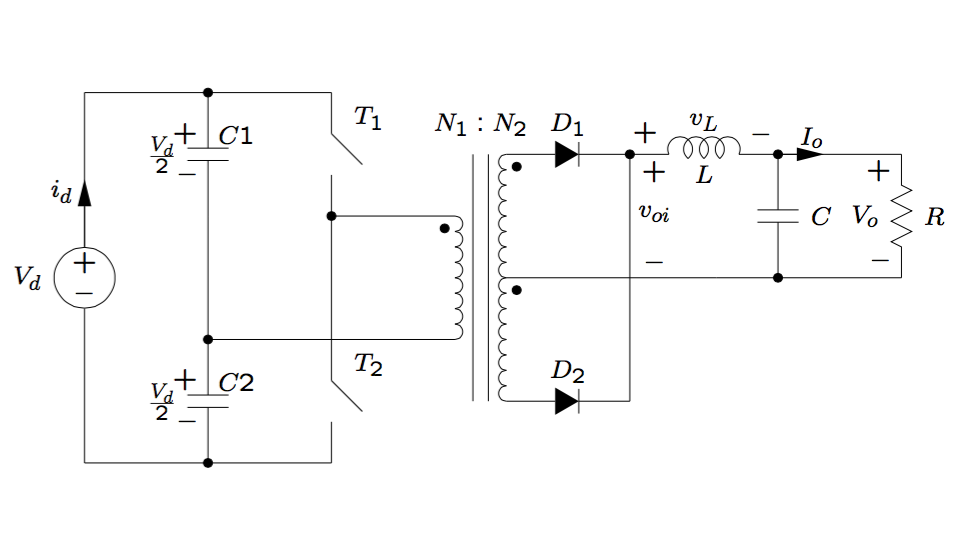
\includegraphics[width=0.8\textwidth, height = 0.5\textwidth]{circ.png}
\caption{Circuit diagram of the half-bridge power supply. Credit Prof. DT. Mouton}
\label{default}
\end{center}
\end{figure}

\begin{table}[htdp]
\caption{Half-Bridge Power Supply Specifications}
\begin{center}
\begin{tabular}{|c|c|c|}
\hline
Parameter & Symbol & Value \\
\hline\hline
Input Voltage & $V_d$ & 30 V \\
\hline
Ouput Voltage & $V_o$ & 15 V \\
\hline
Duty Cycle & $D$ & $\frac{1}{3}$ \\
\hline
Load Current & $I_o$ & 1 A \\
\hline
Switching Frequency & $f_s$ & 50 kHz \\
\hline
Filter Inductance & $L$ & 2mH \\
\hline
Filter Capacitance  & $C$ & 1 000 $\mu$F \\
\hline
\end{tabular}
\end{center}
\label{Half-Bridge Power Supply Specifications}
\end{table}%
\newpage
%%%%%%%%%%%%%%%%%%%%%%%%%%%%%%%%%%%%%%%%%%%%%%%%%%%%%%%%%%%%%%%%%%%%%%%%
\subsection{Theoretical Analysis}
%%%%%%%%%%%%%%%%%%%%%%%%%%%%%%%%%%%%%%%%%%%%%%%%%%%%%%%%%%%%%%%%%%%%%%%%
\subsubsection{Number of Primary Turns of the Transformer}
Faraday's law explained the relationships between voltage and the rate if change of the flux and is more formally defined as follows:
\begin{equation}
v = NA_c\frac{dB}{dt},
\end{equation}
The voltage $v$ is directly proportional to the number of turns $N$, the effective core area $A_c$ as well as the rate of change of the flux {B}. The number of primary turns $N$ is required to be calculated provided that the maximum flux density is 200 mT (with a zero average over a switching cycle). \\
Considering that the voltage has a direct relation to the rate of change of the flux, it is custom to consider the voltage of the primary winding $v = v_1$ initially.   
\begin{figure}[h]
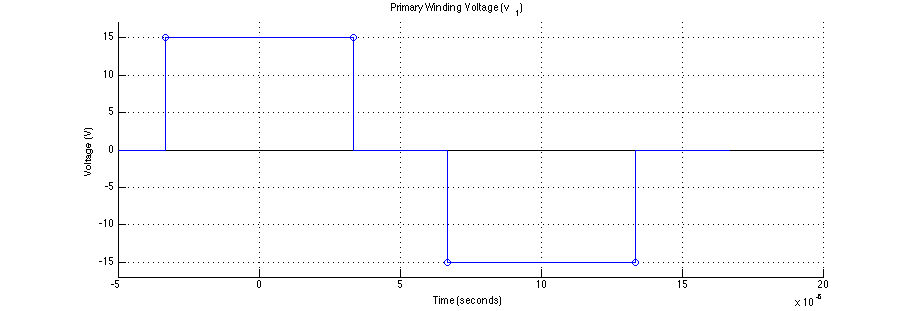
\includegraphics[width=\textwidth, height = 0.35\textwidth]{vp.png}
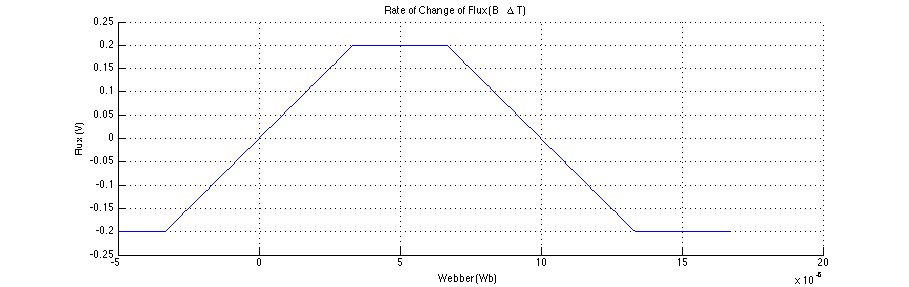
\includegraphics[width=\textwidth, height = 0.35\textwidth]{flux.png}
\caption{Voltage of the Primary Winding and The Rate of Change of Flux}
\label{default}
\end{figure}

Hereafter, it is evident from the figures above that the number of primary turns $N_1$, can be solved from equation (1) as follows:
\begin{equation}
\begin{split}
2B_{max} &=  \frac{v_1}{N_1A_c}\Delta T \\ 
N_1 &= \frac{v_1}{2B_{max}A_c}\Delta T \\
&= \frac{V_d}{4B_{max}A_c}D T_s \\
&= \frac{30}{4(83\times10^{-6})(0.2)}(6.67\times10^{-6}) \\
&=  3.012\hspace{0.2cm}\text{Turns}\\
&= 4\hspace{0.2cm}\text{Full Turns} 
\end{split}
\end{equation}  
%%%%%%%%%%%%%%%%%%%%%%%%%%%%%%%%%%%%%%%%%%%%%%%%%%%%%%%%%%%%%%%%%%%%%%%%
\subsubsection{Number of Secondary Turns of the Transformer}
The relationship between the input and output voltage can be defined as follows in order to determine the windings on the secondary transformer:
\begin{equation}
\begin{split}
\bigg(\frac{N_2}{N_1}\frac{V_d}{2}-V_o\bigg)DT_s &=  V_o\bigg(\frac{1}{2}-D\bigg)T_s\\ 
\therefore N_2 &= 6\hspace{0.2cm}\text{Turns}
\end{split}
\end{equation}  
%%%%%%%%%%%%%%%%%%%%%%%%%%%%%%%%%%%%%%%%%%%%%%%%%%%%%%%%%%%%%%%%%%%%%%%%
\newpage
\section{Practical 3: Control of the Half Bridge Power Supply}
Practical 3 requires the student to extend the design and analysis of the previously designed half-bridge power supply in practical 2. The previously mentioned specifications are thus extended to incorporate the effects of parasitic resistances. In short, as the duty-cycle approaches unity, the inductor current sufficiently increases causing major losses. The extended design of the power supply possesses the following additional specifications to this of the previous practical:  

\begin{table}[htdp]
\caption{Extended Half-Bridge Power Supply Specifications}
\begin{center}
\begin{tabular}{|c|c|c|}
\hline
Parameter & Symbol & Value \\
\hline\hline
Equivalent Series Resistance (Inductor) & $r_L$ & 0.6 $\Omega$ \\
\hline
Equivalent Series Resistance (Capacitor) & $r_C$ & 0.05 $\Omega$ \\
\hline
\end{tabular}
\end{center}
\label{Half-Bridge Power Supply Specifications}
\end{table}%
With regard to the functionality of the power supply, it is required that a control loop be set up from the output of the power supply to the input of the pulse width modulator (PWM). This control loop is then modelled accordingly in order to set up a transfer function. The goal is to then derive a state-variable representation of the circuit according to each of the switching states. This will allow the circuit to be simulated in software so that the behaviour can be sufficiently analysed (with the effect of parasitic resistances taken into account). The closed loop controller is shown as follows: 

\begin{figure}[h]
\begin{center}
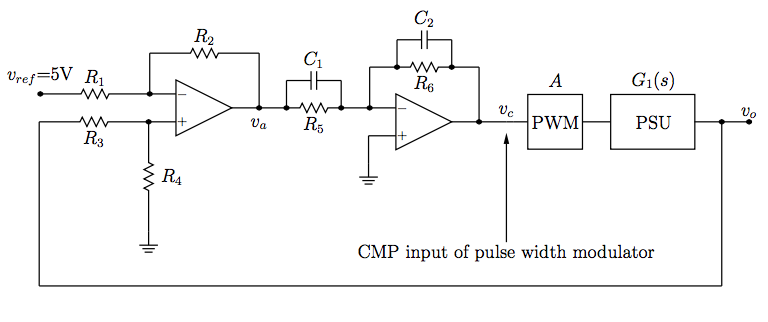
\includegraphics[width=0.9\textwidth, height = 0.45\textwidth]{prac3.png}
\caption{Circuit diagram of control loop. Credit Prof. DT. Mouton}
\label{default}
\end{center}
\end{figure}
\newpage
%%%%%%%%%%%%%%%%%%%%%%%%%%%%%%%%%%%%%%%%%%%%%%%%%%%%%%%%%%%%%%%%%%%%%%%%
\subsection{Theoretical Analysis: Transfer Function}
\subsubsection{State Variable Representation}
The linearisation technique of Middlebrow and C\`{u}k is used and subsequently adjusted/modified to determine the transfer function of the power supply output with respect to the duty-cycle (control input):\\\\
Assuming that the state variable description over a switching period is taken as the average values, the state variable representation is defined as follows,\\
\begin{equation}
\begin{split}
\textbf{\.{x}} &= [\textbf{A}_1d+\textbf{A}_2(1-d)]\textbf{x}+[\textbf{B}_1d+\textbf{B}_2(1-d)]V_d \\
		   &= \frac{2}{T_s}\Big[[\textbf{A}_1dT_s+\textbf{A}_2(0.5-d)T_s]\textbf{x}+[\textbf{B}_1dT_s+\textbf{B}_2(0.5-d)T_s]V_d\Big] \\
		   &= 2[\textbf{A}_1d+\textbf{A}_2(0.5-d)]\textbf{x}+2[\textbf{B}_1d+\textbf{B}_2(0.5-d)]V_d \\
		   &= \textbf{A}_1\textbf{x}+2\textbf{B}_1dV_d
\end{split}
\end{equation}

with $\textbf{A}_1 = \textbf{A}_2$ and $\textbf{B}_2 = [0\hspace{0.15cm}0]^T$.\\\\
The output is similarly derived:
\begin{equation}
\begin{split}
{v}_o  &= \frac{2}{T_s}\Big[[\textbf{C}_1dT_s+\textbf{C}_2(0.5-d)T_s]\textbf{x}]\Big]\\
&= \textbf{C}_1\textbf{x}
\end{split}
\end{equation}
with $\textbf{C}_1 = \textbf{C}_2$.
%%%%%%%%%%%%%%%%%%%%%%%%%%%%%%%%%%%%%%%%%%%%%%%%%%%%%%%%%%%%%%%%%%%%%%%%
\subsubsection{Model Dynamics}
In order to completely define the dynamics of the system, it is necessary to model the dynamics of the system in order to define the transition model of the state-variable representation. This process involves modelling the dynamics (setting up the differential equations that describe the system) of the system and writing them in state space format. This format is derived as follows:\\\\
The state variable are chosen as the capacitor voltage $v_C(t)$ and the inductor current $i_L(t)$,
\begin{equation}
\begin{split}
 \frac{N_2}{N_1} \frac{V_d}{2} &= L \frac{di_L(t)}{dt} + r_L i_L(t) + v_C(t) + C\frac{dv_C(t)}{dt} r_C\\
 v_C(t) &+ C\frac{dv_C(t)}{dt} r_C = R\bigg(i_L(t)-C\frac{dv_C(t)}{dt}\bigg)
\end{split}
\end{equation}
In order to obtain the state variables in matrix form, it is required that they are the subject of the formula:
\begin{equation}
\begin{split}
\frac{di_L(t)}{dt} &= - \frac{1}{L}\bigg( \frac{R r_L + r_Cr_L + r_CR}{R+r_c}\bigg)i_L(t) - \frac{1}{L}\bigg(\frac{R}{R+r_c}\bigg)v_C(t)+ \frac{N_2}{N_1} \frac{V_d}{2} \\
\frac{dv_C(t)}{dt} &= \frac{R}{C(R+r_c)}i_L(t)-\frac{1}{C(R+r_c)}v_C(t)
\end{split}
\end{equation}
The output voltage $v_o(t)$ can equivalently be derived as follows:
\begin{equation}
\begin{split}
v_o &= R\bigg(i_L(t) -C\frac{dv_C(t)}{dt} \bigg) \\
&= R\bigg(i_L(t) -\frac{R}{R+r_c}i_L(t)+\frac{R}{R+r_c}v_C(t)\bigg)\\
&= \frac{Rr_c}{R+r_c}i_L(t)+\frac{R}{R+r_c}v_C(t)
\end{split}
\end{equation}
Now the entire model can be represented in matrix form,
%%%%%%%%%%%%%%%%%%%%%%%%%%%%%
\begin{equation}
\begin{split}
 \begin{bmatrix}
\frac{di_L(t)}{dt} \\
 \frac{dv_C(t)}{dt}\\
 \end{bmatrix}  &= 
 \begin{bmatrix}
 - \frac{1}{L}\bigg( \frac{R r_L + r_Cr_L + r_CR}{R+r_c}\bigg) & - \frac{1}{L}\bigg(\frac{R}{R+r_c}\bigg) \\
 \frac{R}{C(R+r_c)} 								       & -\frac{1}{C(R+r_c)} \\
 \end{bmatrix} 
  \begin{bmatrix}
i_L(t) \\
v_C(t)\\
\end{bmatrix}
+   \begin{bmatrix}
\frac{N_2}{N_1} \frac{1}{2L} \\
0\\
\end{bmatrix} V_d \\
%%%%%%%%%%%%%%%%%%%%%%%%%%%%%%%%%%%
&\approx 
 \begin{bmatrix}
 - \frac{1}{L}(r_L + r_C) & - \frac{1}{L} \\
 \frac{1}{C} & -\frac{1}{RC} \\
 \end{bmatrix} 
  \begin{bmatrix}
i_L(t) \\
v_C(t)\\
\end{bmatrix}
+   \begin{bmatrix}
\frac{N_2}{N_1} \frac{1}{2L} \\
0\\
\end{bmatrix} V_d
\end{split}
\end{equation}
with the aforementioned approximation as a result of the assumption that $r_C << R$ and $r_L << R$.\\\\
Finally the output in matrix form is shown as follows:
\begin{equation}
\begin{split}
v_o &= \begin{bmatrix}
 \frac{Rr_c}{R+r_c}i_L(t) & \frac{R}{R+r_c}v_C(t)\\
\end{bmatrix}
\begin{bmatrix}
i_L(t) \\
v_C(t)\\
\end{bmatrix}+
\begin{bmatrix}
0\\
0\\
\end{bmatrix}V_d \\
&\approx \begin{bmatrix}
 r_C & 1\\
\end{bmatrix}
\begin{bmatrix}
i_L(t) \\
v_C(t)\\
\end{bmatrix}+
\begin{bmatrix}
0\\
0\\
\end{bmatrix}V_d \\
\end{split}
\end{equation}
%%%%%%%%%%%%%%%%%%%%%%%%%%%%%%%%%%%%%%%%%%%%%%%%%%%%%%%%%%%%%%%%%%%%%%%%
\subsubsection{Laplace Transform}
The state-variable representation represents a set of differential equations and can thus be Laplace Transformed for convenience sake:
\begin{equation}
\begin{split}
s\textbf{X}(s)  &= \textbf{A}_1\textbf{X}(s)+2\textbf{B}_1V_d\hspace{0.1cm}d(s) \\
(s\textbf{I}-\textbf{A}_1)\textbf{X}(s)&= 2\textbf{B}_1V_d\hspace{0.1cm}d(s) \\
\textbf{X}(s) &= (s\textbf{I}-\textbf{A}_1)^{-1}2\textbf{B}_1V_d\hspace{0.1cm}d(s) \\\\
V_o(s) &= \textbf{C}_1\textbf{X}(s)\\
&=  \textbf{C}_1(s\textbf{I}-\textbf{A}_1)^{-1}2\textbf{B}_1V_d\hspace{0.1cm}d(s)
\end{split}
\end{equation}
The transfer function can then be defined as the ratio between the input $\textbf{d}(s)$ and the output $\textbf{V}_o(s)$:
\begin{equation}
\begin{split}
G_1(s)  &= \frac{v_o(s)}{d(s)} = \textbf{C}_1(s\textbf{I}-\textbf{A}_1)^{-1}2\textbf{B}_1V_d \\
&= \frac{\textbf{C}_1(s\textbf{I}-\textbf{A}_1)^{-1}2\textbf{B}_1V_d}{|s\textbf{I}-\textbf{A}_1|}
\end{split}
\end{equation}
The transfer function can then be defined in terms of the model dynamics described in the previous section:
\begin{equation}
\begin{split}
G_1(s)  &= \cfrac{\begin{bmatrix}
r_C & 1 \\
\end{bmatrix}
\begin{bmatrix}
s + \frac{1}{RC} & - \frac{1}{L}\\
\frac{1}{C} & s + \frac{1}{L}(r_C + r_L)\\
\end{bmatrix}2
\begin{bmatrix}
\frac{N_2}{N_1} \frac{1}{2L} \\
0\\
\end{bmatrix}V_d}
{s^2 +\Big(\frac{1}{RC}+\frac{1}{L}(r_L+r_C)\Big)s + \frac{1}{RLC}(r_L+r_C) + \frac{1}{LC}} \\
&= \frac{\frac{N_2}{N_1} \frac{V_d}{L}(sr_C+\frac{r_C}{RC}+\frac{1}{C})}{s^2 +\Big(\frac{1}{RC}+\frac{1}{L}(r_L+r_C)\Big)s + \frac{1}{RLC}(r_L+r_C) + \frac{1}{LC}} \times \frac{C}{C} \\
&\equiv \frac{N_2}{N_1} V_d \Bigg[\frac{1+sr_C C}{LC\big(s^2 +\big(\frac{1}{RC}+\frac{1}{L}(r_L+r_C)\big)s + \frac{1}{LC}\big)}\Bigg].
\end{split}
\end{equation}
%%%%%%%%%%%%%%%%%%%%%%%%%%%%%%%%%%%%%%%%%%%%%%%%%%%%%%%%%%%%%%%%%%%%%%%%
\newpage
\subsection{Theoretical Analysis: Difference Amplifier}
With reference to figure 4 above, it can be observed that the feedback loop is connected to a difference amplifier with a reference voltage $v_{ref}$ and an output voltage of $v_a$. It is required that the output voltage be represented in terms of the reference voltage.\\

\begin{figure}[h]
\begin{center}
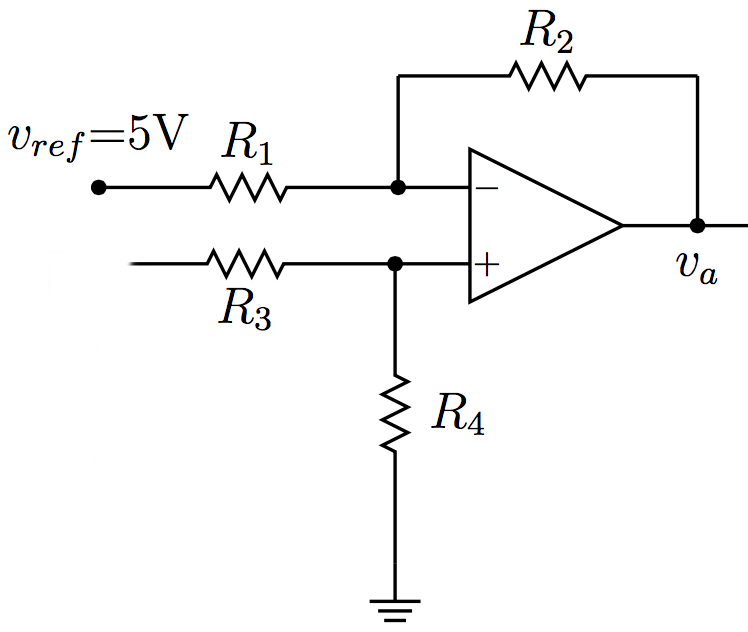
\includegraphics[width=0.5\textwidth, height = 0.4\textwidth]{diffAmp.png}
\caption{Circuit diagram of the difference amplifier. Credit Prof. DT. Mouton}
\label{default}
\end{center}
\end{figure}
Assuming that a virtual short circuit exists between the positive and negative terminals of the operational amplifier, the node voltage analysis can be described as follows:
\begin{equation}
\begin{split}
\frac{V^{-}-v_{ref}}{R_1} + \frac{V^{-}-v_a}{R_2} &= 0 \\
\frac{V^{+}-v_o}{R_3} + \frac{V^{+}}{R_4} &= 0
\end{split}
\end{equation}
defining $V^+ = V^- = \frac{v_o}{R_3}\Big(\frac{R_3R_4}{R_3+R_4}\Big)=\Big(\frac{R_4}{R_3+R_4}\Big)v_o$ it can be deduced that,
\begin{equation}
\begin{split}
\frac{R_4}{R_1}\Big(\frac{1}{R_3+R_4}\Big)&v_o - \frac{V_{ref}}{R_1}+\frac{R_4}{R_2}\Big(\frac{1}{R_3+R_4}\Big)v_o - \frac{v_a}{R_2} = 0 \\
v_a &= R_2R_4\Bigg(\frac{R_1 + R_2}{R_2R_1(R_3+R_4)}\Bigg)v_o - \frac{R_2}{R_1}v_{ref} \\
v_a &= -\frac{R_2}{R_1}v_{ref} + \Bigg(\frac{\frac{1}{R_4}}{\frac{1}{R_4}} \frac{\frac{1}{R_1}}{\frac{1}{R_1}}\Bigg) \frac{1+\frac{R_2}{R_1}}{1+\frac{R_3}{R_4}}v_o \\
v_a &\equiv -\frac{R_2}{R_1}v_{ref} + \frac{1+\frac{R_2}{R_1}}{1+\frac{R_3}{R_4}}v_o
\end{split}
\end{equation}
\newpage
%%%%%%%%%%%%%%%%%%%%%%%%%%%%%%%%%%%%%%%%%%%%%%%%%%%%%%%%%%%%%%%%%%%%%%%%
\subsection{Theoretical Analysis: Lead Compensator}
A lead compensator aims to improve an undesirable frequency response in a feedback control system. By introducing a pole-zero pair (typically near the origin) into the open loop transfer function, the compensator should provide a phase lag at low frequencies and reduce steady state error. The lead compensator circuit in this practical is shown as follows in the figure below:

\begin{figure}[h]
\begin{center}
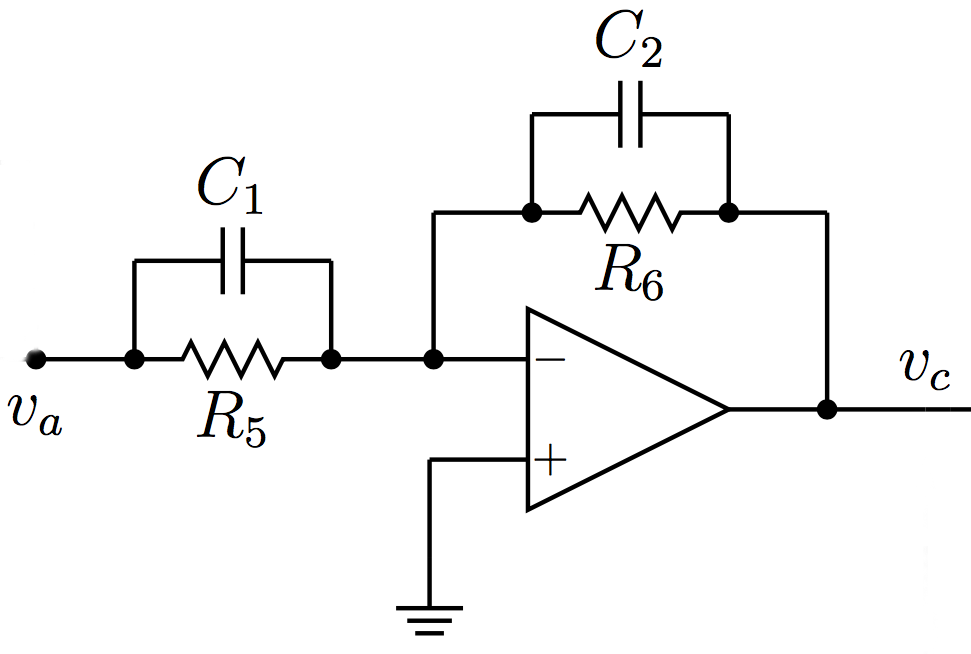
\includegraphics[width=0.5\textwidth, height = 0.4\textwidth]{lead.png}
\caption{Circuit diagram of the lead compensator. Credit Prof. DT. Mouton}
\label{default}
\end{center}
\end{figure}
Assuming that the capacitors are represented as $\frac{1}{sC}$ in the Laplace-domain. It is required to determine the transfer function of the lead compensator. This can be achieved by a node voltage analysis at the negative terminal of the operational amplifier:
\begin{equation}
\begin{split}
\cfrac{0-v_{a}}{\cfrac{R_5\frac{1}{sC_1}}{\frac{1}{sC_1}+R_5}} + \cfrac{0-v_c}{\cfrac{R_6\frac{1}{sC_2}}{\frac{1}{sC_2}+R_6}} &= 0 \\
-\Bigg(\cfrac{1+sC_1R_5}{R_5}\Bigg)v_a - \Bigg(\cfrac{1+sC_1R_6}{R_6}\Bigg)v_c&= 0
\end{split}
\end{equation}
The transfer function $G_2(s)$ can be defined as the ration between the input to the lead compensator $v_a$ and its output $v_c$:
\begin{equation}
\begin{split}
G_2(s) &= \cfrac{v_c}{v_a} =\cfrac{\Bigg(\cfrac{1+sC_1R_5}{R_5}\Bigg)}{\Bigg(\cfrac{1+sC_1R_6}{R_6}\Bigg)}\equiv -\cfrac{C_1}{C_2}\cfrac{\frac{1}{C_1R_5}+s}{\frac{1}{C_1R_6}+s}
\end{split}
\end{equation}
%%%%%%%%%%%%%%%%%%%%%%%%%%%%%%%%%%%%%%%%%%%%%%%%%%%%%%%%%%%%%%%%%%%%%%%
\subsection{Simulation: Transfer Function}
The theoretical predictions can be adequately simulated through software packages (in this case MATLAB) in order to successfully simulate the behaviour of the aforementioned theoretical system/s. It can be recalled that the transfer function of the power supply $G_1(s)$, is represented as the following second order system:
\begin{equation}
\begin{split}
G_1(s) &= \frac{N_2}{N_1} V_d \Bigg[\frac{1+sr_C C}{LC\big(s^2 +\big(\frac{1}{RC}+\frac{1}{L}(r_L+r_C)\big)s + \frac{1}{LC}\big)}\Bigg]
\end{split}
\end{equation}
This second order system yields the following frequency response:

\begin{figure}[h]
\begin{center}
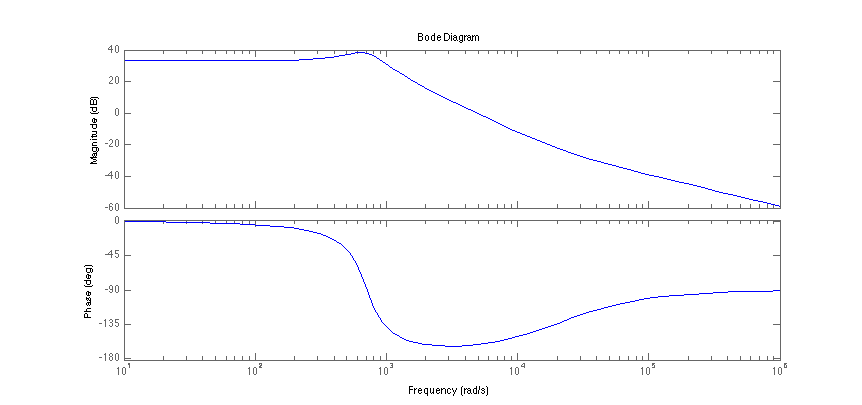
\includegraphics[width=\textwidth, height = 0.7\textwidth]{bode1.png}
\caption{Frequency response of the transfer function $G_1(s)$}
\label{default}
\end{center}
\end{figure} 
\newpage
%%%%%%%%%%%%%%%%%%%%%%%%%%%%%%%%%%%%%%%%%%%%%%%%%%%%%%%%%%%%%%%%%%%%%%%%
\subsection{Simulation: Lead Compensator}
Initially the lead compensator is assumed to have a unity gain after which it is required than root locus be sketched for an open loop system comprising of the PWM, power supply and a lead compensator with the following specifications:
\begin{equation}
\begin{split}
G_2(s) &= \frac{s+2000\pi}{s+4000\pi}
\end{split}
\end{equation}
The resulting root locus for the aforementioned system, $G(s)=G_1(s)G_2(s)$, is as follows (open loop characteristics (left) and closed loop characteristics (right)):

\begin{figure}[h]
\begin{center}
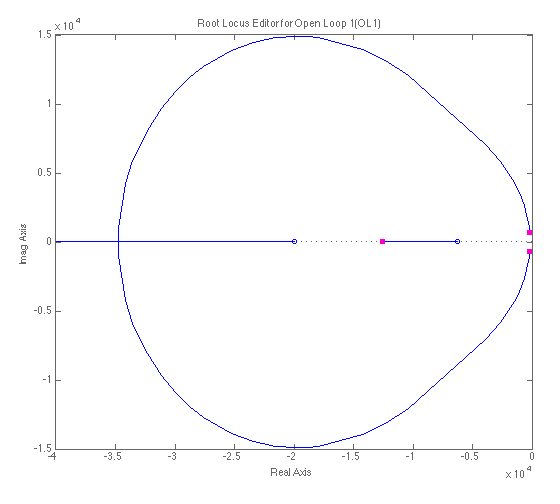
\includegraphics[width=0.49\textwidth, height = 0.6\textwidth]{q6.png}
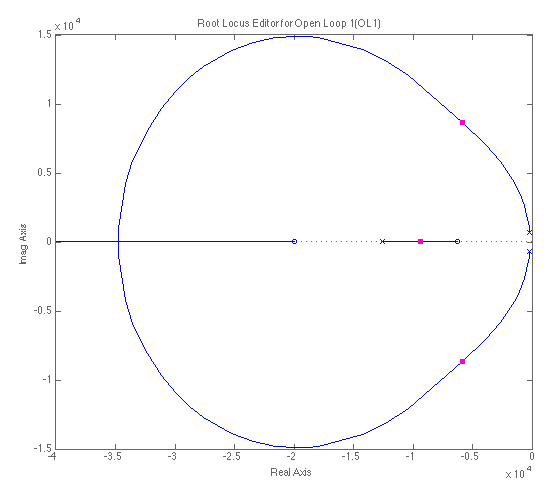
\includegraphics[width=0.49\textwidth, height = 0.6\textwidth]{q7.png}
\caption{Root locus of the system  (open loop (left) and closed loop (right))}
\label{default}
\end{center}
\end{figure} 
where 'x' denotes an open loop poles, 'o' denotes an open loop zero and the pink square denotes the closed loop poles.\\\\
In order to obtain a desired damping ratio - 0.559 in this specific case - a set of two complex closed loop poles are to be inserted. The placement of these poles will yield the desired damping ration and additionally cause a 12\% overshoot in the step response of the system accordingly. The "rltool" in MATLAB is successfully used in order to find the desired location of the closed loop poles on the locus. These locations can be observed form figure 7 above (left).   
\newpage
%%%%%%%%%%%%%%%%%%%%%%%%%%%%%%%%%%%%%%%%%%%%%%%%%%%%%%%%%%%%%%%%%%%%%%%%
The aforementioned case of the desired damping ratio requires an additional gain of approximately 36.3 (determined form MATLAB). In order to realise this in the system relevant in this practical, the previously assumed unity gains of the lead compensator as well as the differential amplifier are to be adjusted accordingly to obtain the desired gain. Once achieved, the required gain will yield a step response of the system with a zero steady-state tracking error. The step response of the system is shown as follows:

\begin{figure}[h]
\begin{center}
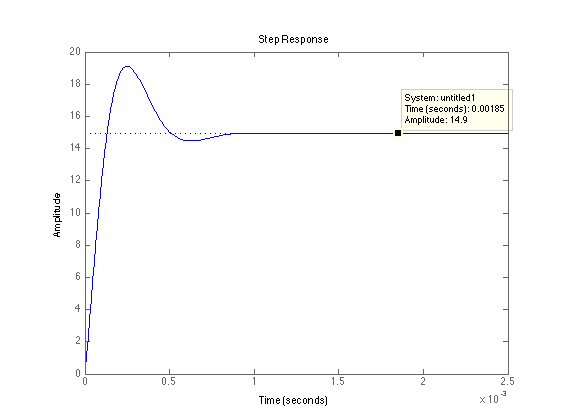
\includegraphics[width=0.8\textwidth, height = 0.6\textwidth]{sse.png}
\caption{Root locus of the system  (open loop (left) and closed loop (right))}
\label{default}
\end{center}
\end{figure}  
The theoretical steady-state error can be calculated as follows:
\begin{equation}
\begin{split}
e_{ss} (\infty) &= \frac{1}{1+\lim_{s\rightarrow0}G(s)}=\frac{1}{1+K_{p}} \\
&= \frac{1}{1+9} = 0.1\\
&\therefore K_{p}=\lim_{s\rightarrow0}G(s)= 9 \\
\end{split}
\end{equation}
The simulation in MATLAB supports these calculations as can be seen from figure 8 above wit a steady-state error of 0.1. \\\\
%%%%%%%%%%%%%%%%%%%%%%%%%%%%%%%%%%%%%%%%%%%%%%%%%%%%%%%%%%%%%%%%%%%%%%%%
\subsection{Component Design}
As previously mentioned, the gains of both the differential amplifier as well as the lead compensator are to be tuned in order to achieve the required gain of 36.3 (to adhere to the steady-state specifications). In order to tune these gains, the component values are free to be adjusted accordingly. The choices for the gains of each individual component are as follows:\\
\begin{center}
$\frac{C_1}{C_2} = 3.63$ and  $ \frac{1+\frac{R_2}{R_1}}{1+\frac{R_3}{R_4}} = K_2 = 10$
\end{center}

Whilst still adhering to the general dynamics of the differential amplifier, the design is undertaken as follows:
\begin{equation}
\begin{split}
v_a = -\Bigg(\frac{R_2}{R_1}\Bigg)v_{ref} &+ \Bigg(\frac{1+\frac{R_2}{R_1}}{1+\frac{R_3}{R_4}}\Bigg)v_o = 0 \\
-5K_1 &= -15K_2 \\
K_1 &= 3\times K_2
\end{split} 
\end{equation}
where 
\begin{center}
$K_1 = \frac{R_2}{R_1} = 30$ and $K_2 = \frac{1+\frac{R_2}{R_1}}{1+\frac{R_3}{R_4}} = 10$
\end{center}
This implies that a choice can be made regarding resistors $R_1$ and $R_4$ as well as capacitors $C_1$ and $C_2$, provided that the desired gain of 36.3 is still achieved. The following choices are then made for the aforementioned components.

\begin{table}[htdp]
\caption{Lead Compensator and Differential Amplifier Component Specifications}
\begin{center}
\begin{tabular}{|c|c|c|}
\hline
Parameter & Symbol & Value \\
\hline\hline
Resistor & $R_1$ & 1 k$\Omega$ \\
\hline
Resistor & $R_4$ & 1 k$\Omega$ \\
\hline
Capacitor & $C_1$ & 33 nF \\
\hline
Capacitor & $C_2$ & 10 nF \\
\hline
\end{tabular}
\end{center}
\label{Half-Bridge Power Supply Specifications}
\end{table}%
Hereafter, the remainder of the component values can be calculated as follows:\\
\begin{equation}
\begin{split}
R_2 &= K_1 \times R_1 = 30 k\Omega \\
R_3 &= R_4\bigg(\frac{1+K_1}{K_2} - 1\bigg) = 2.1 k\Omega\\
R_5 &= \frac{1}{2\pi(1000)C_1} = 4.548 k\Omega \\
R_6 &= \frac{1}{2\pi(2000)C_2} = 7.958 k\Omega
\end{split} 
\end{equation}
\newpage
%%%%%%%%%%%%%%%%%%%%%%%%%%%%%%%%%%%%%%%%%%%%%%%%%%%%%%%%%%%%%%%%%%%%%%%%
%%%%%%%%%%%%%%%%%%%%%%%%%%%%%%%%%%%%%%%%%%%%%%%%%%%%%%%%%%%%%%%%%%%%%%%%
%%%%%%%%%%%%%%%%%%%%%%%%%%%%%%%%%%%%%%%%%%%%%%%%%%%%%%%%%%%%%%%%%%%%%%%%
%%%%%%%%%%%%%%%%%%%%%%%%%%%%%%%%%%%%%%%%%%%%%%%%%%%%%%%%%%%%%%%%%%%%%%%%
%%%%%%%%%%%%%%%%%%%%%%%%%%%%%%%%%%%%%%%%%%%%%%%%%%%%%%%%%%%%%%%%%%%%%%%%
















\end{document}  